\documentclass{article}

\usepackage[margin=1in]{geometry}
\usepackage{amsmath}
\usepackage{graphicx}

% Redefining maketitle to adjust the title font size
\makeatletter
\renewcommand{\maketitle}{\bgroup\setlength{\parindent}{0pt}
\begin{flushleft}
  \textbf{\LARGE \@title} \\ % Change \LARGE to desired size if needed
  \vspace{0.5em}
  \@author
\end{flushleft}\egroup
}
\makeatother

\title{JiaShua - A Complex System Simulation: A Report}
\author{Nan Jia, Joshua Rollins}

\begin{document}
\maketitle
\section*{Abstract}
This report demonstrates the simulation of a complex system. The system is a call center with various random variables that affect the system. The report will show the simulation of the system and the results of the simulation.

\section{Introduction}
This mid-term project is to simulation the call center mechanism. The call center is a complex system with various variables including server state, event calendar, global variables for tracking and measuring performance, and random variables. Those elements aims to mimic a real-life call center scenaio and to provide a way to measure the performance of the call center. The programming language used is \emph{Python}. This report consists of the following sections: system description, simulation method, simulation result, and conclusion.

\section{System Description}
A major auto retailer's call center is examined for its call processing, especially during midday peak times in the upcoming holiday season. When customers call, they connect to a switch. If more than ten calls are on hold, the customer receives a busy tone and hangs up. If not, the call proceeds to an interactive voice response (IVR) unit where callers choose between car-stereo products or other products. The call is then queued according to the product type until a sales representative is available. The goal is to determine the minimum number of sales representatives required to ensure less than 2\% of calls wait more than 1 minute and less than 3% are refused at the switch.

Key assumptions include the instantaneous action of the switch and the IVR unit's capacity to handle multiple calls simultaneously. The IVR involves a pure delay, which must be accounted for. The project employs a physical random number generator using two dice (DICE). This DICE determines various delays and product type requests. For instance, the time between call arrivals is calculated as (DICE * 0.333) minutes. The IVR unit's delay is (DICE * 0.3) minutes, while car-stereo and other product processing times are (DICE * 2) minutes and (DICE) minutes respectively. Lastly, if the DICE rolls a value less than or equal to 4, it's assumed the call is for a car stereo, representing an average 16.7\% of all calls. Otherwise, it's for other products.

\section{Simulation Method}
This section will present the big picture of the simulation as Figure~\ref{fig:call_center}. We start an infinite loop within the main function. When we call this function, the server will be turn on. Then, the program will checking whether it is $4$ pm because the business hours is from $11$ to $4$ that is $300$ minutes. It will directly walk to Event 5: simulation termination. After those system's checking, event calendar will be ready to feed into the core functionality of this call center. 

First, the program will verify whether there is an availbale spot to serve the incoming customer as shown in Figure~\ref{fig:call_center}, the box of Busy Signal. If not, the customer will hang up. Otherwise, the customer will be served by the server. The server will check whether the customer is calling for car stereo or other products. If the customer is calling for car stereo, the server will serve the customer for randome minutes. After the server finishes serving the customer, the server will check whether there is a customer in the queue. If there is a customer in the queue, the server will serve the customer. Otherwise, this representative  will be set available. 
\begin{figure}[t!]
\centering
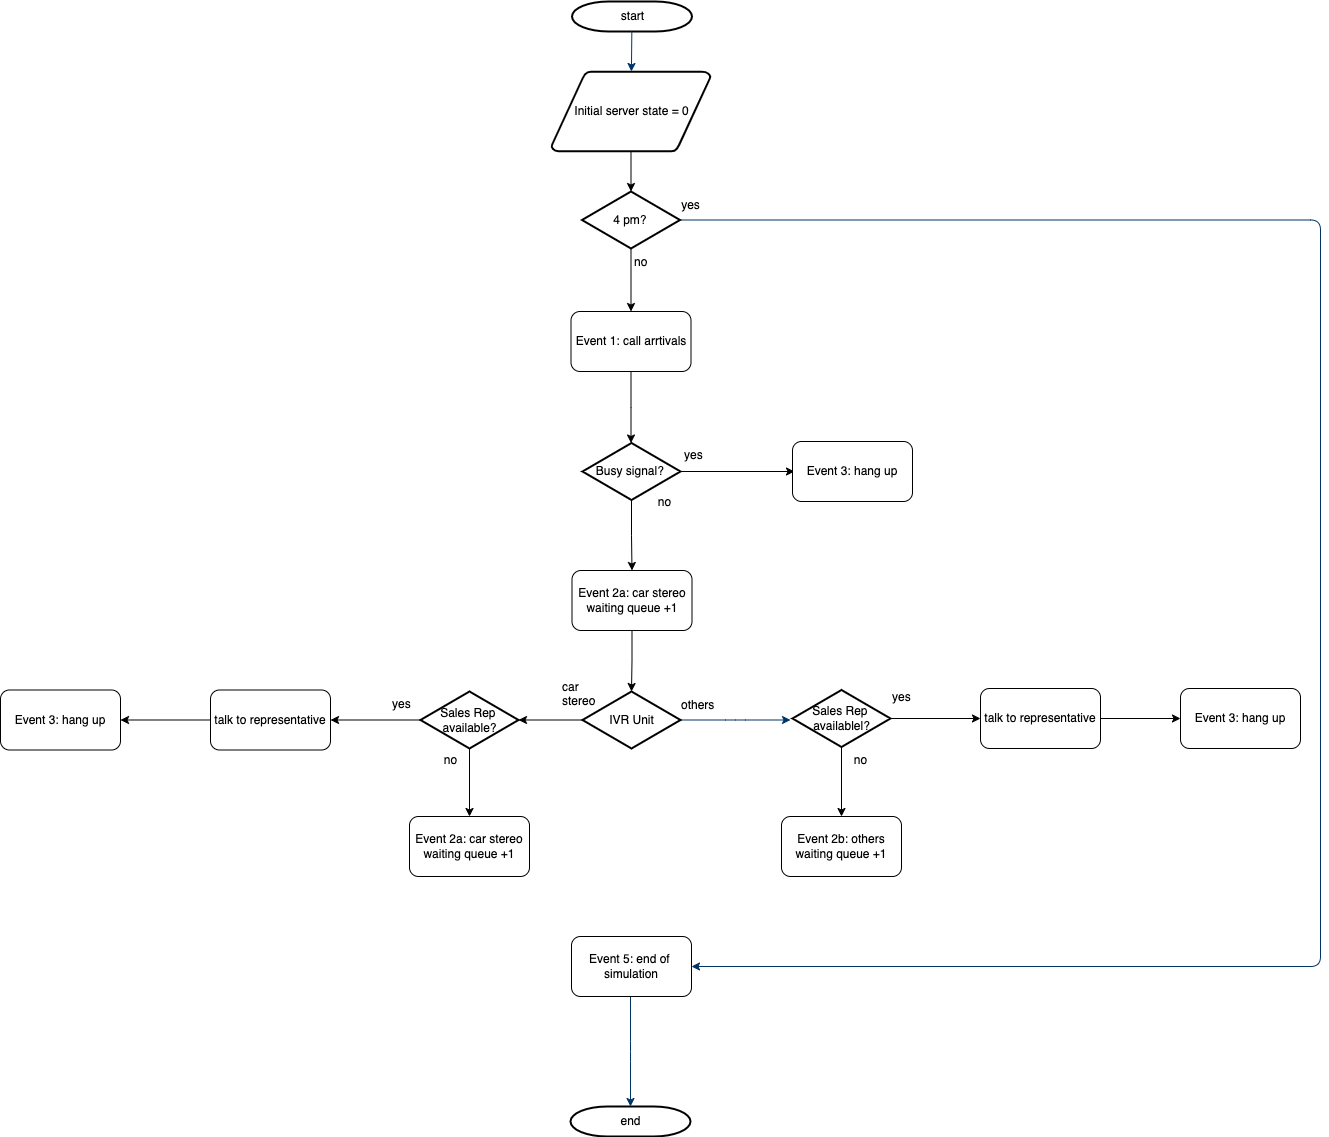
\includegraphics[width=1.1\textwidth]{call_center.png}
\caption{Call Center Controlflow Chart}
\label{fig:call_center}
\end{figure}

\section{Simulation Result}
\section{Conclusion}
\end{document}